\begin{figure}[H]
        \centering
        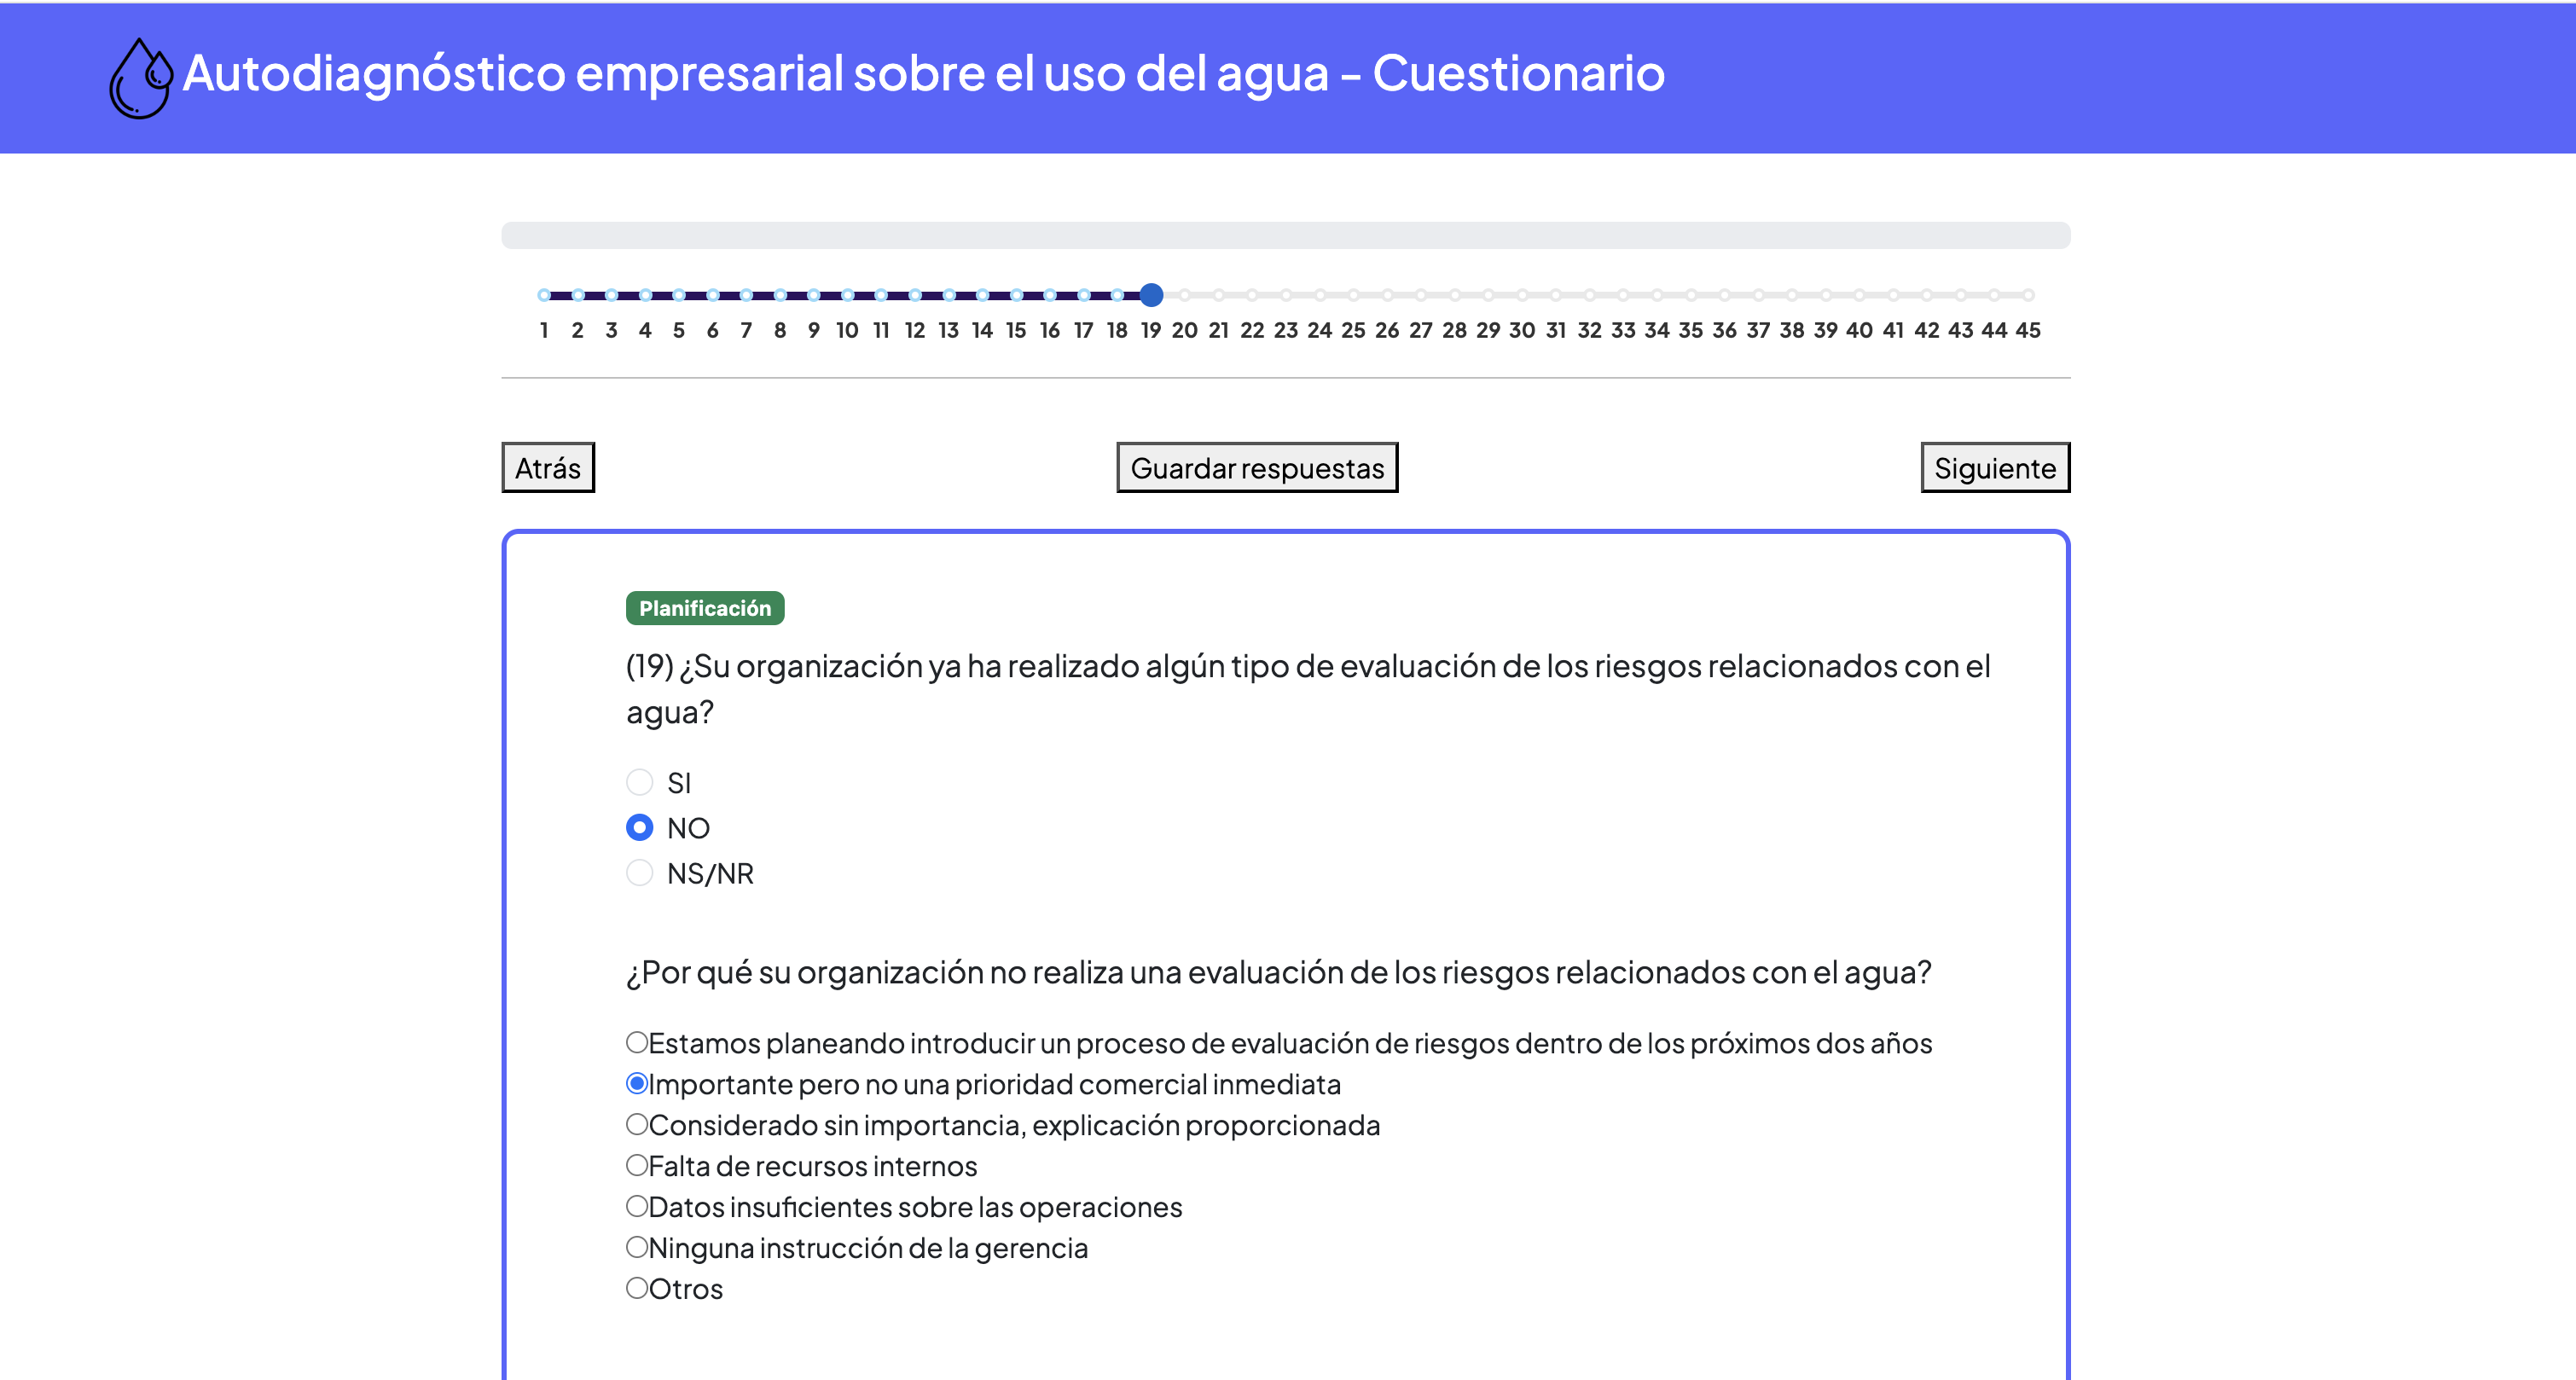
\includegraphics[scale=0.25]{images/99-aplicacion-web/3-cuestionario.png}
        \caption{Pantalla 'Cuestionaro' en la aplicación web}
\end{figure}

\begin{figure}[H]
        \centering
        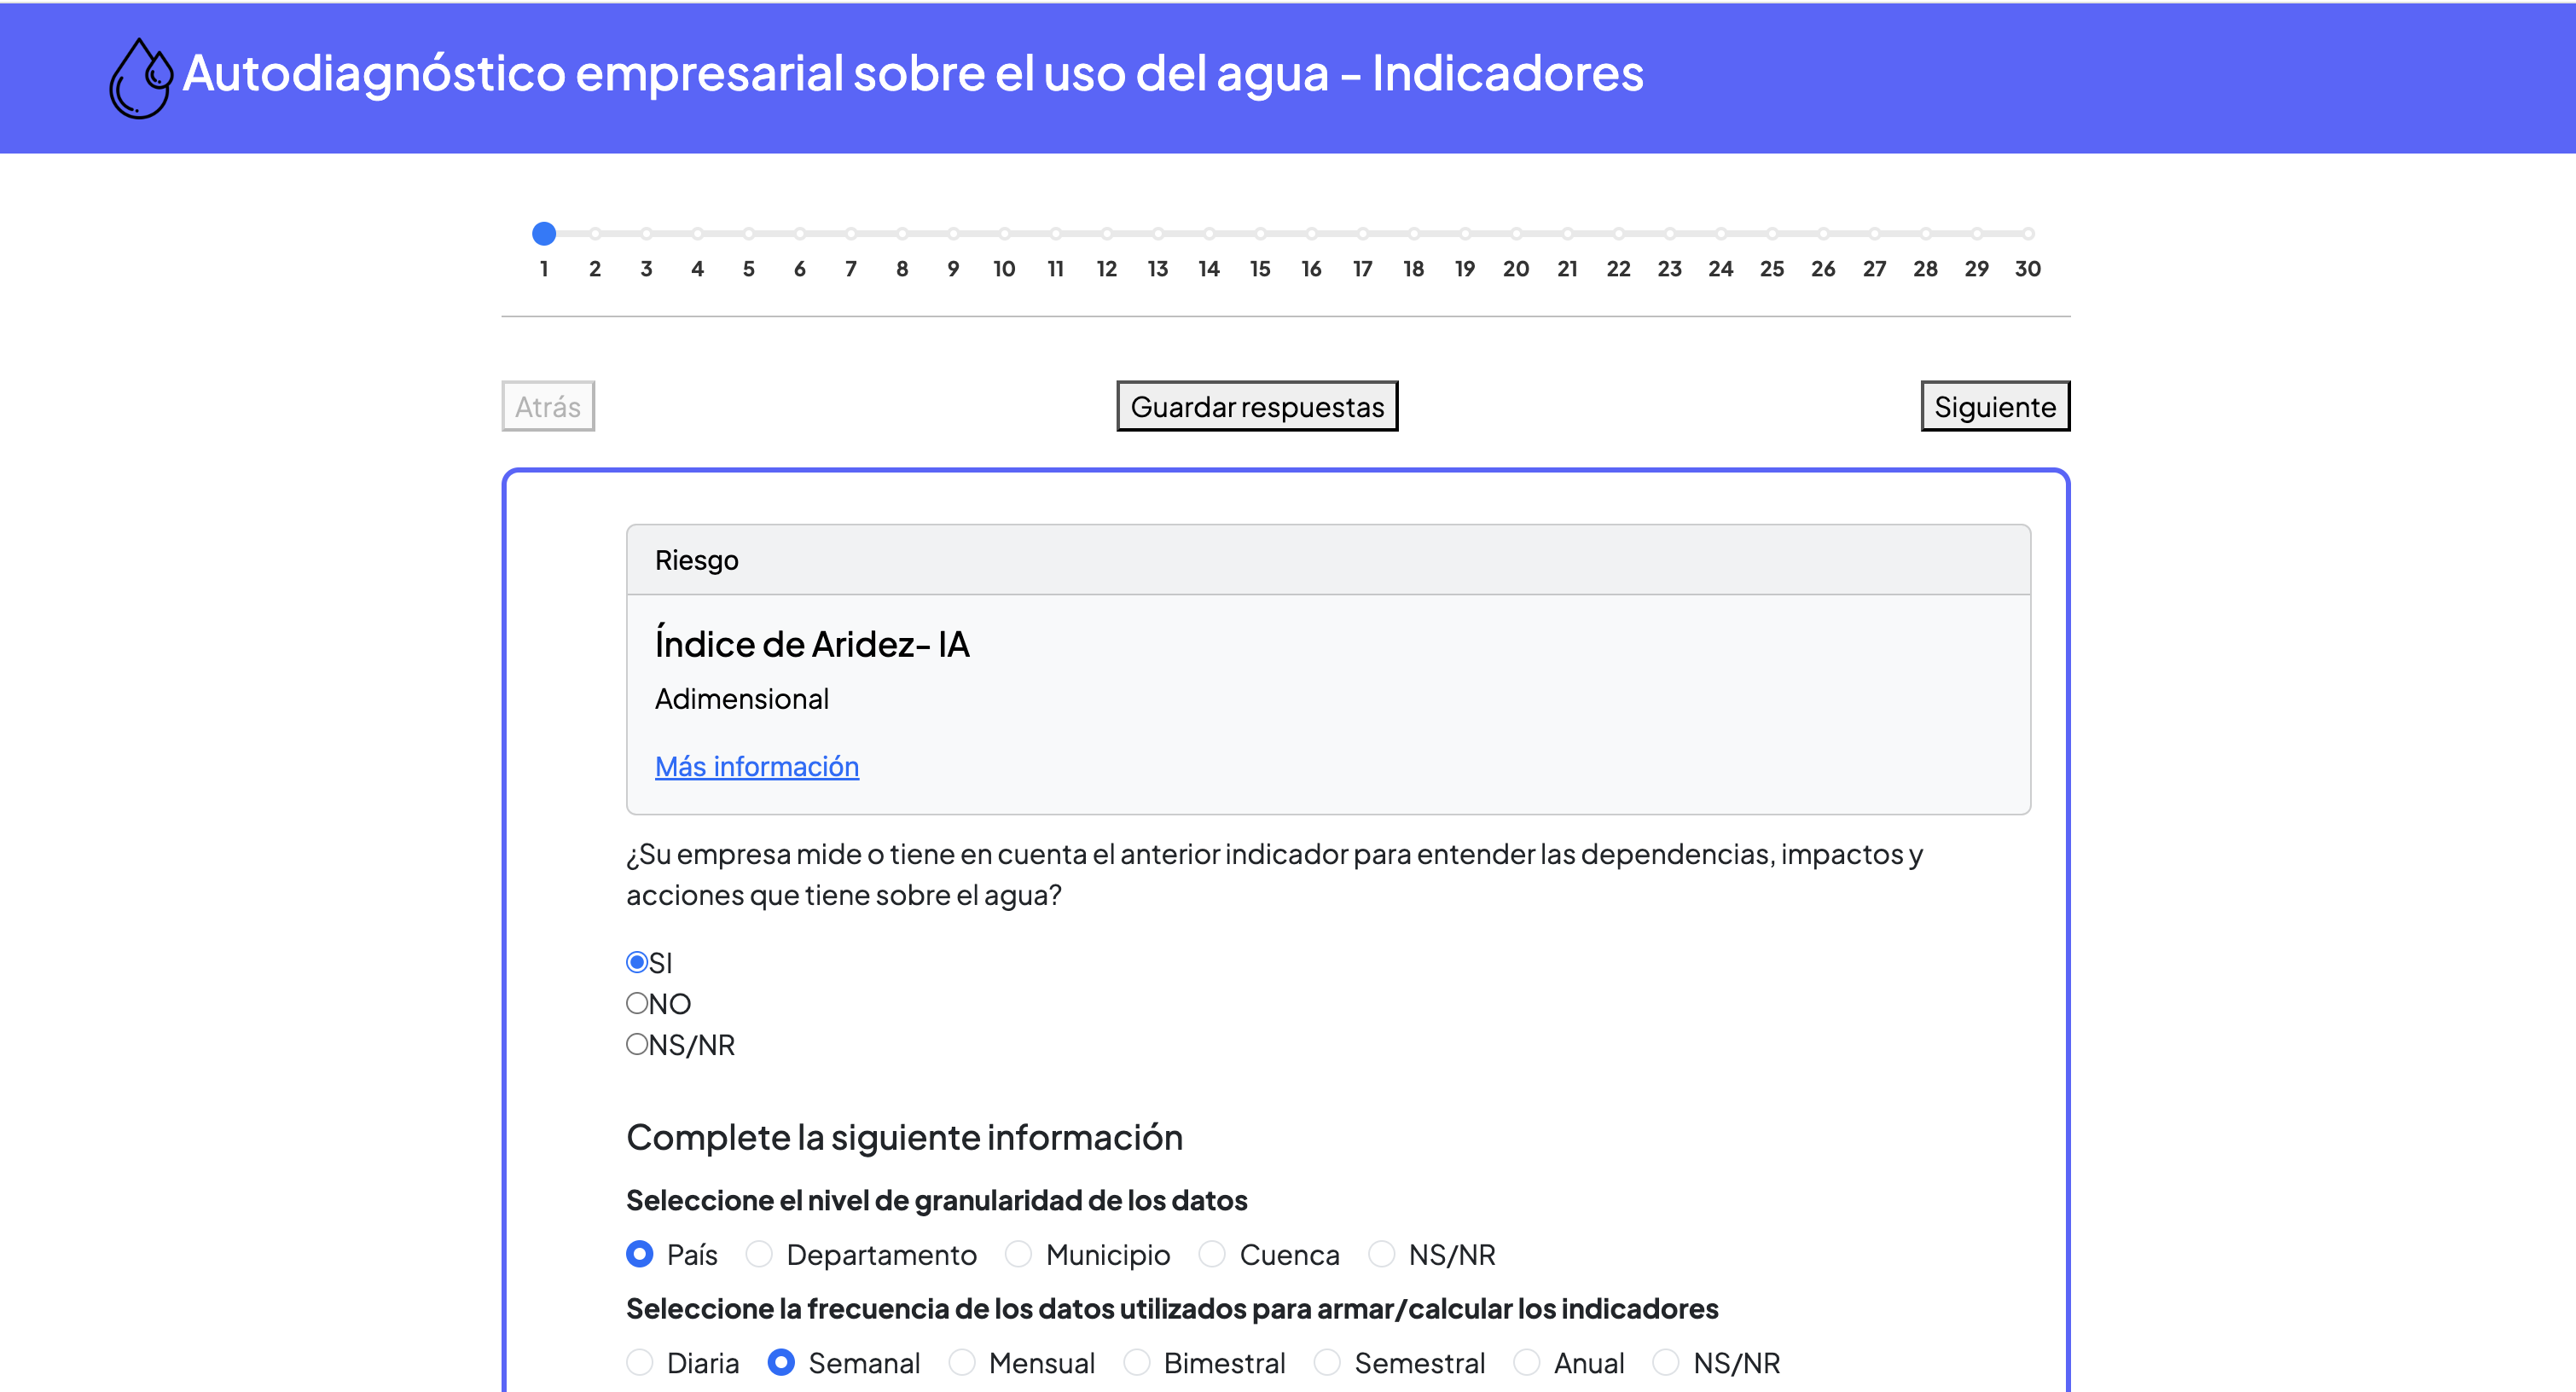
\includegraphics[scale=0.25]{images/99-aplicacion-web/4-indicadores.png}
        \caption{Pantalla 'Indicadores' en la aplicación web}
\end{figure}

\begin{figure}[H]
        \centering
        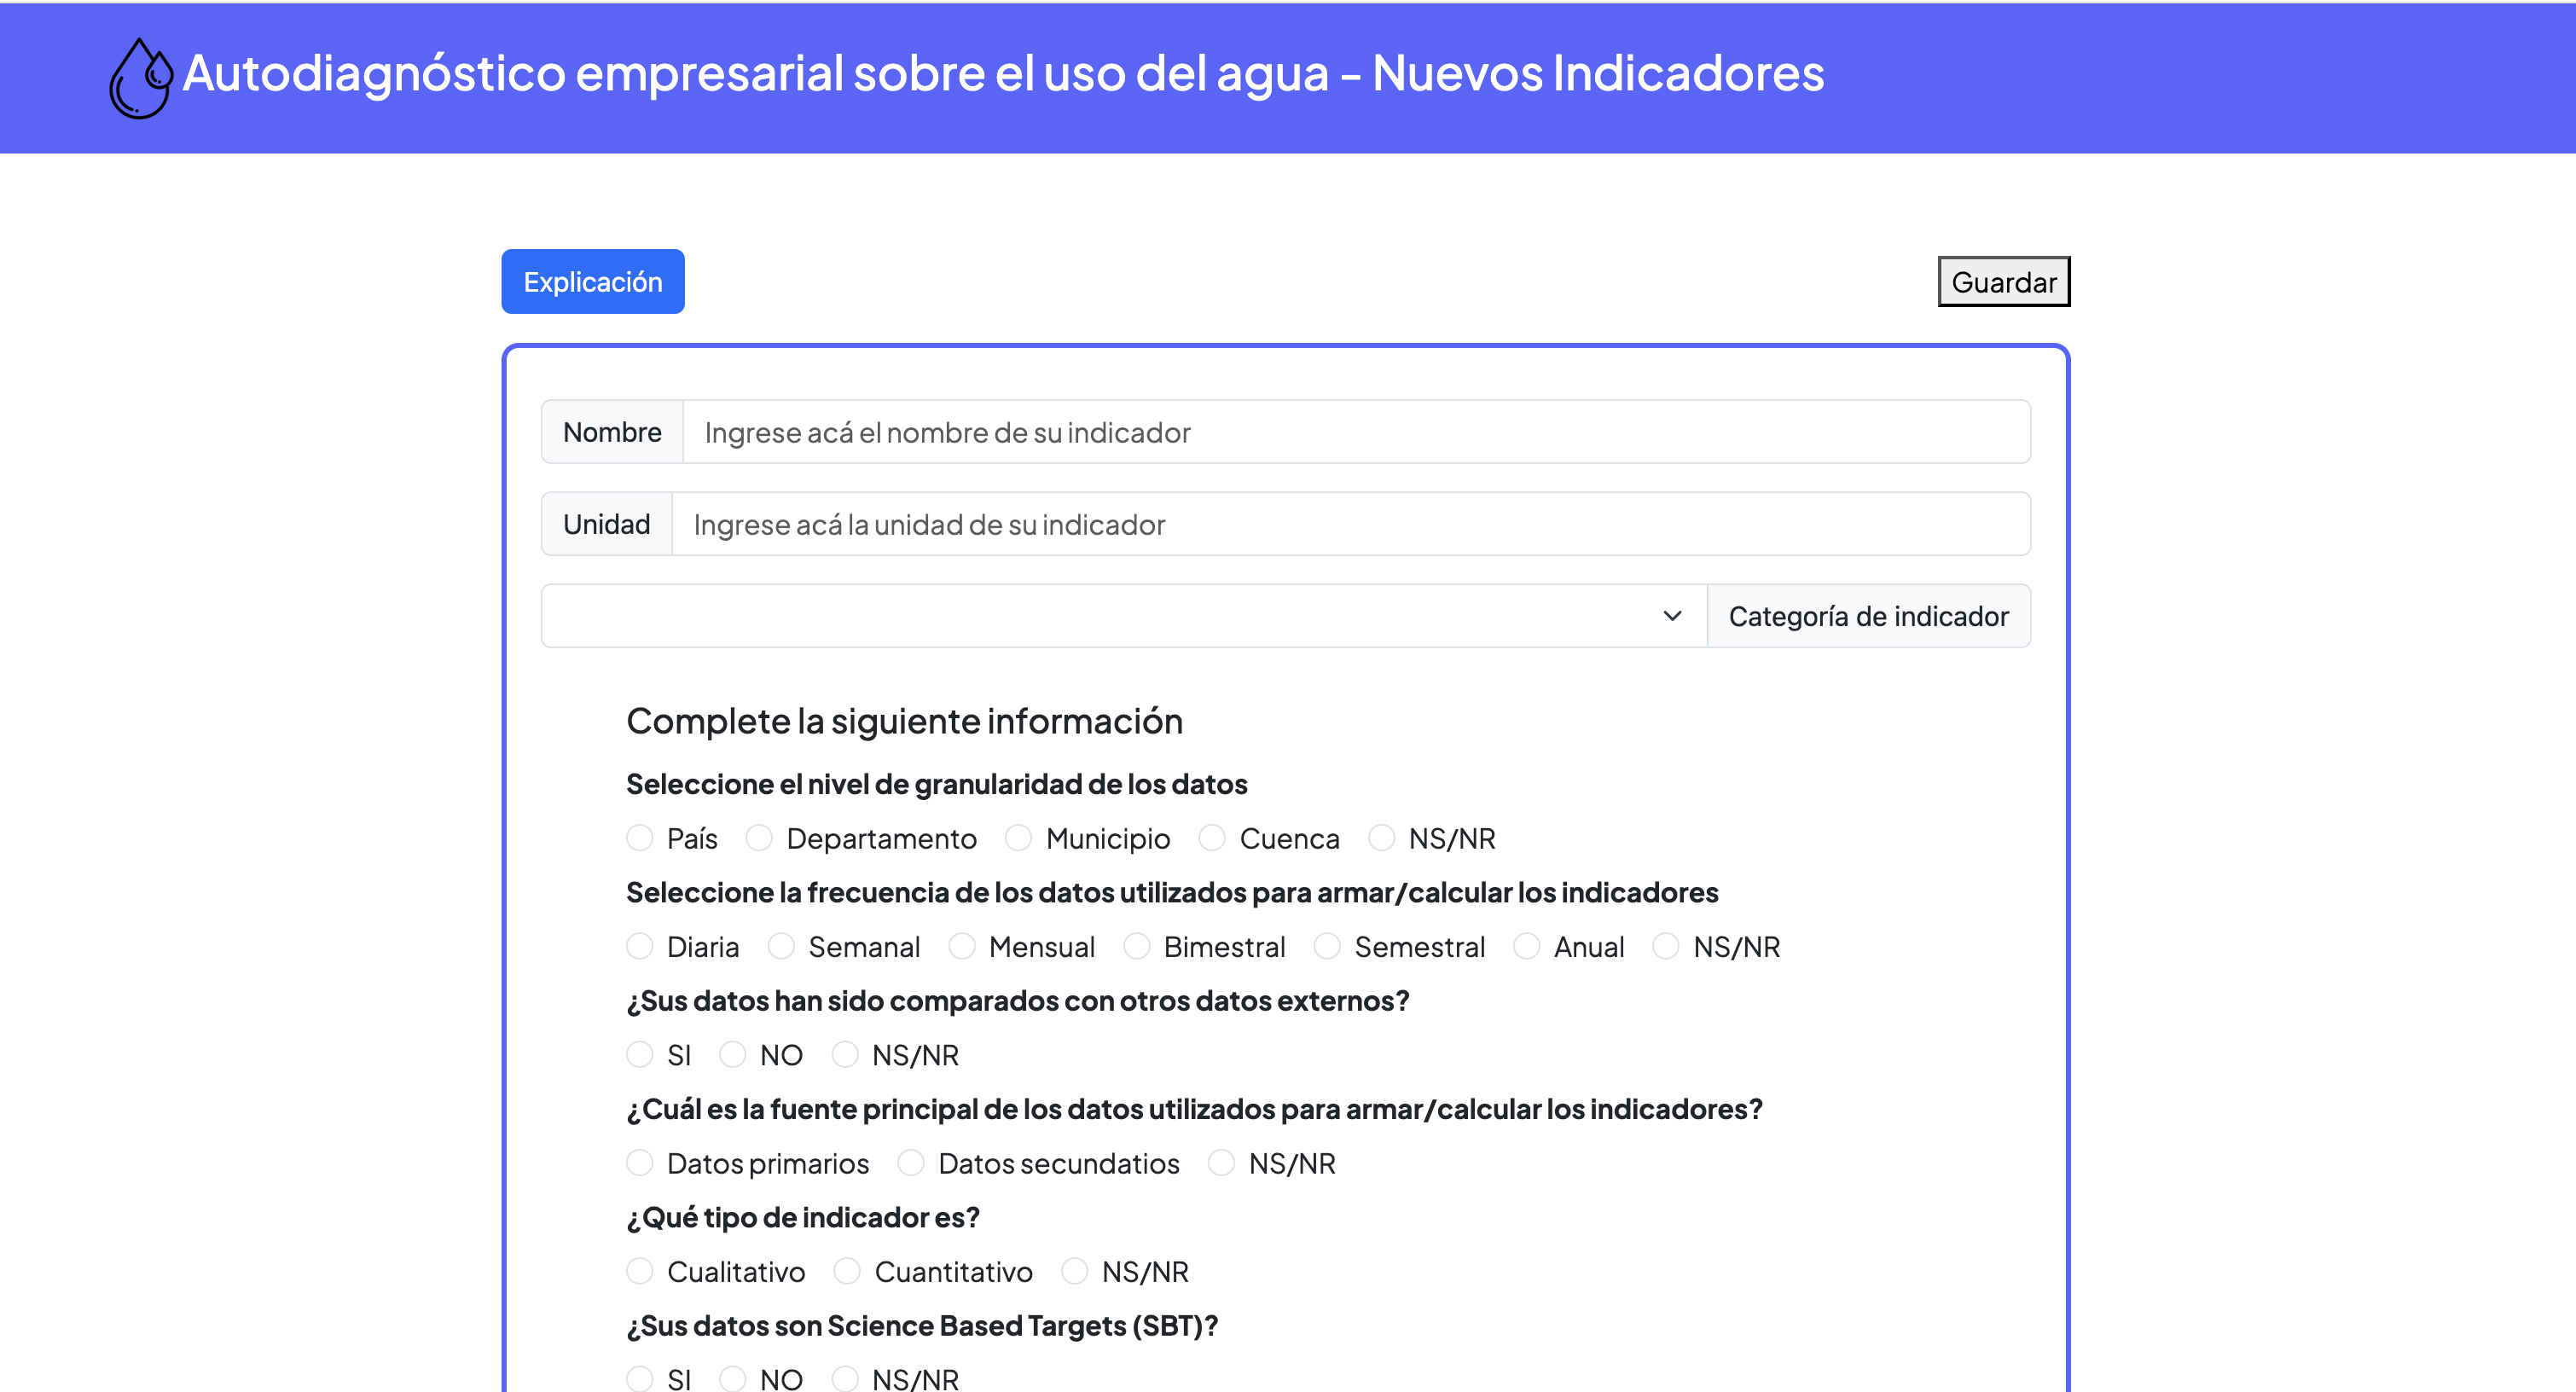
\includegraphics[scale=0.25]{images/99-aplicacion-web/5-nuevos-indicadores.png}
        \caption{Pantalla donde las empresas pueden agregar nuevos indicadores}
\end{figure}

\begin{figure}[H]
        \centering
        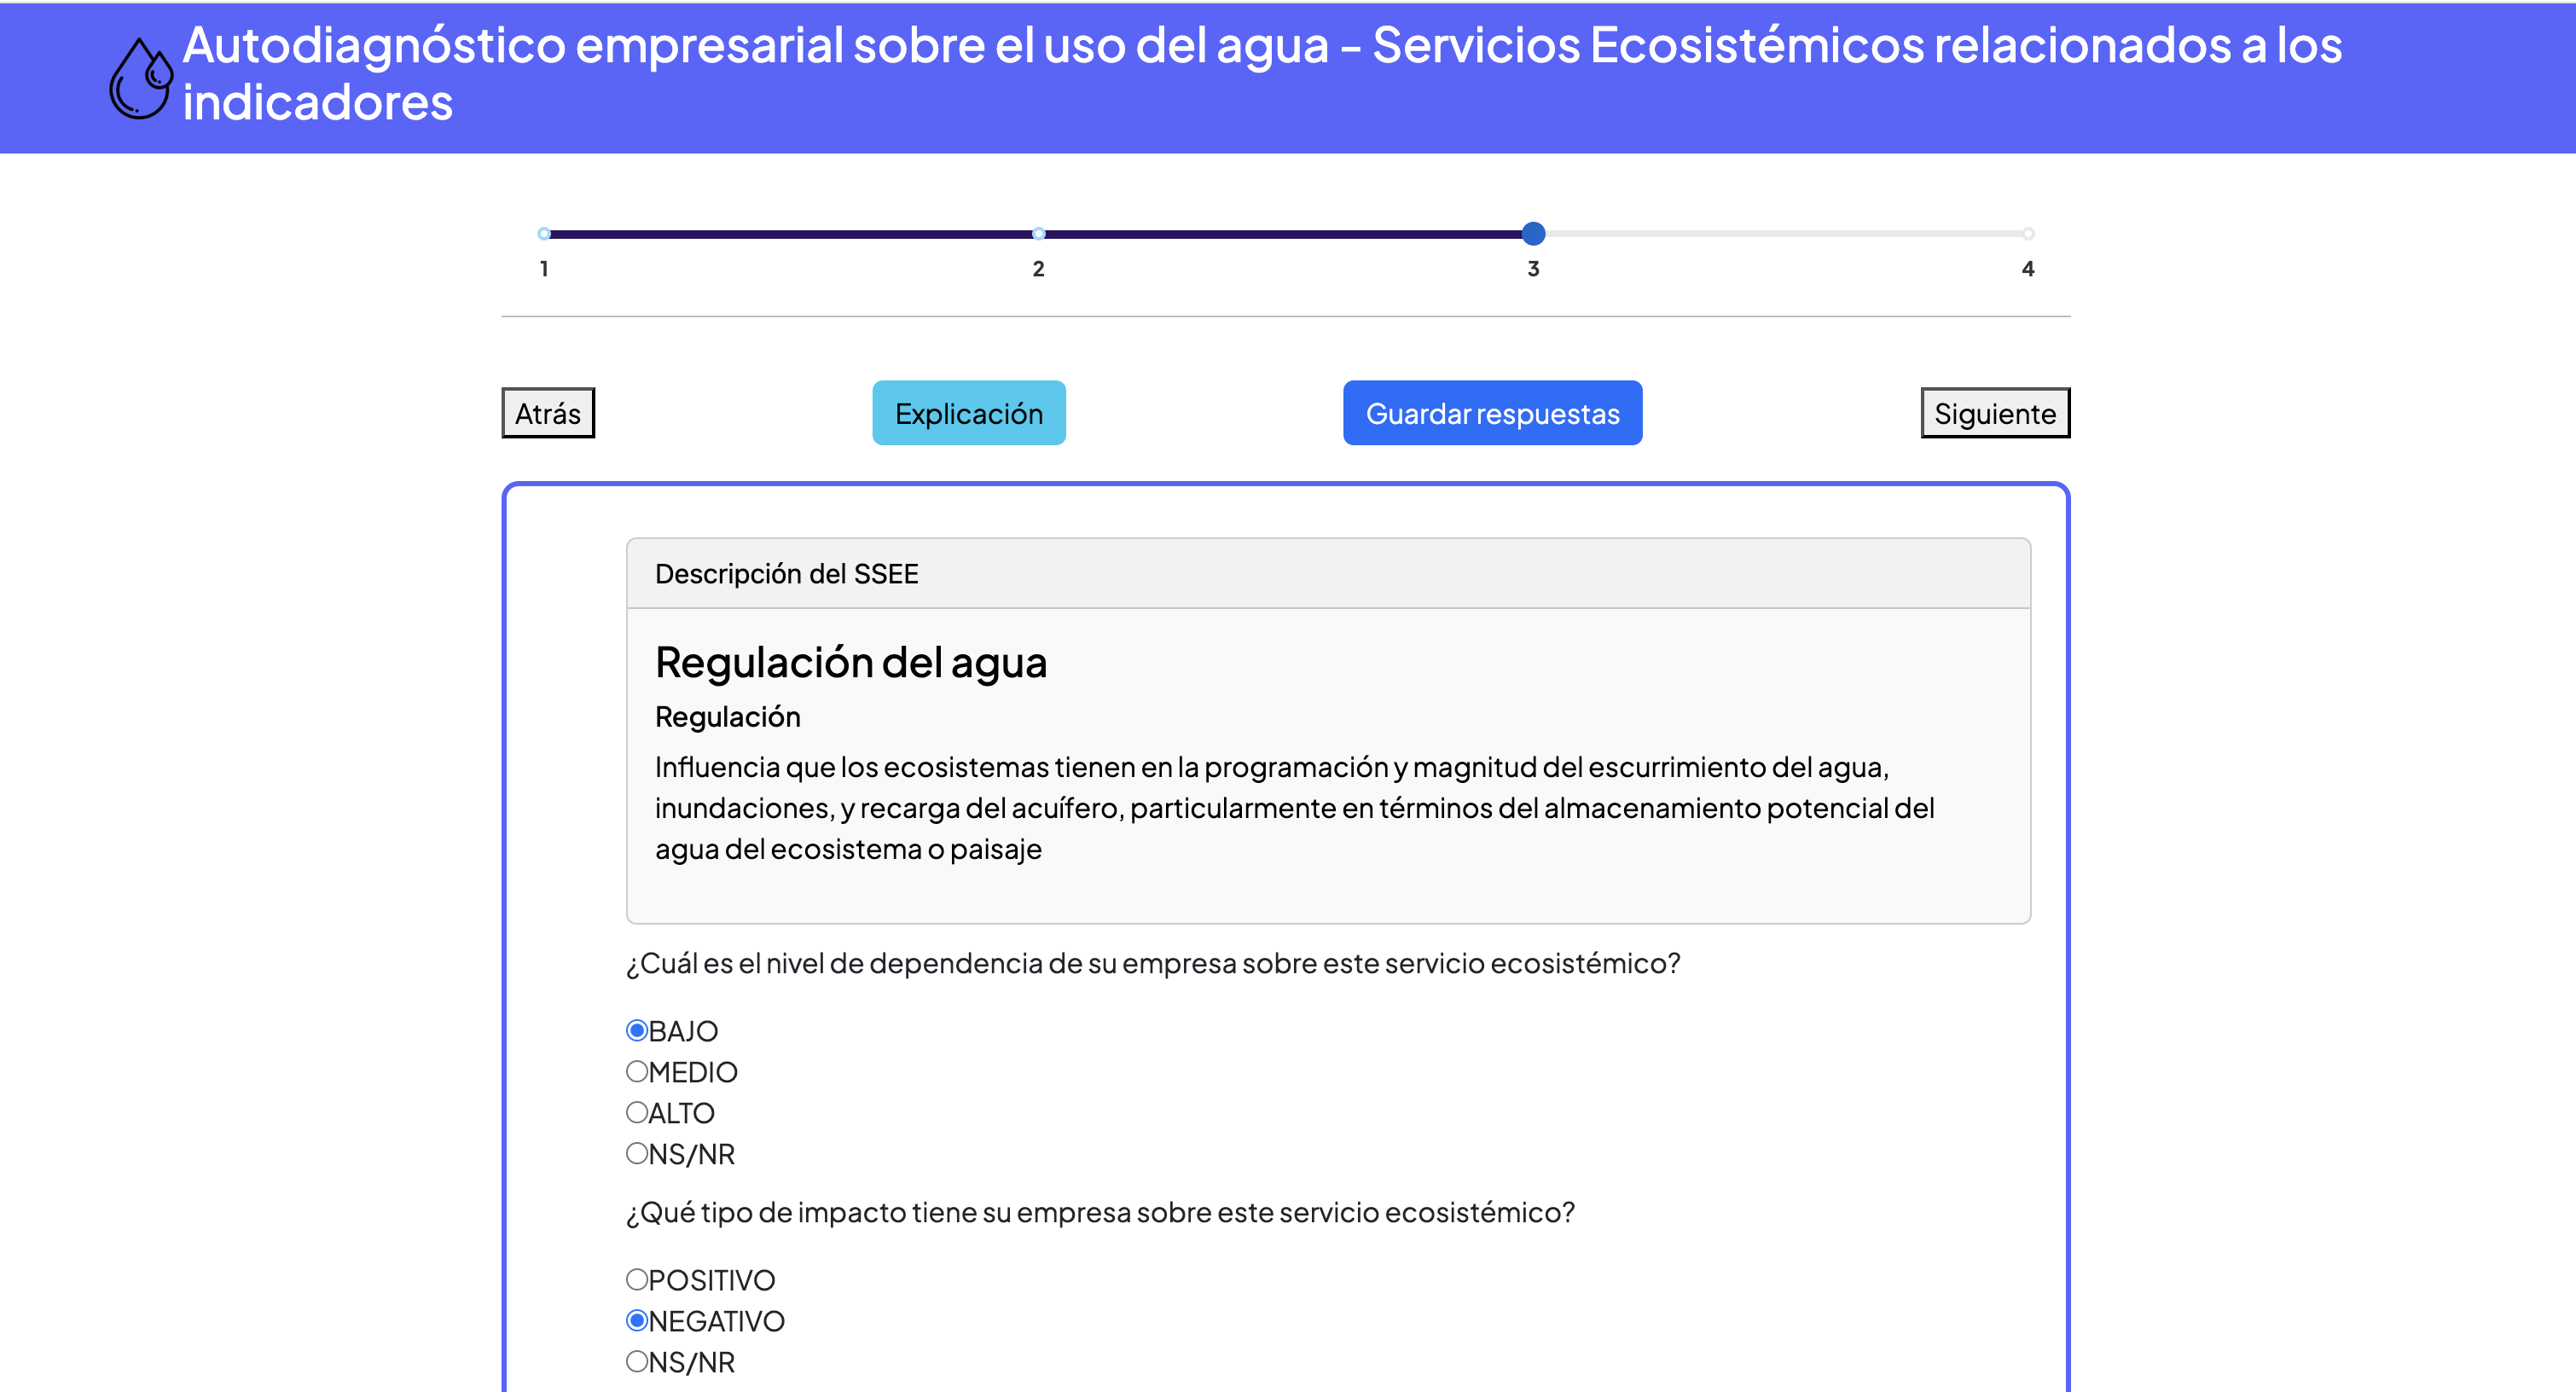
\includegraphics[scale=0.25]{images/99-aplicacion-web/6-ssee.png}
        \caption{Paso donde la empresa determina el nivel de dependencia y el tipo de impacto sobre un servicio ecosistémico}
\end{figure}

\begin{figure}[H]
        \centering
        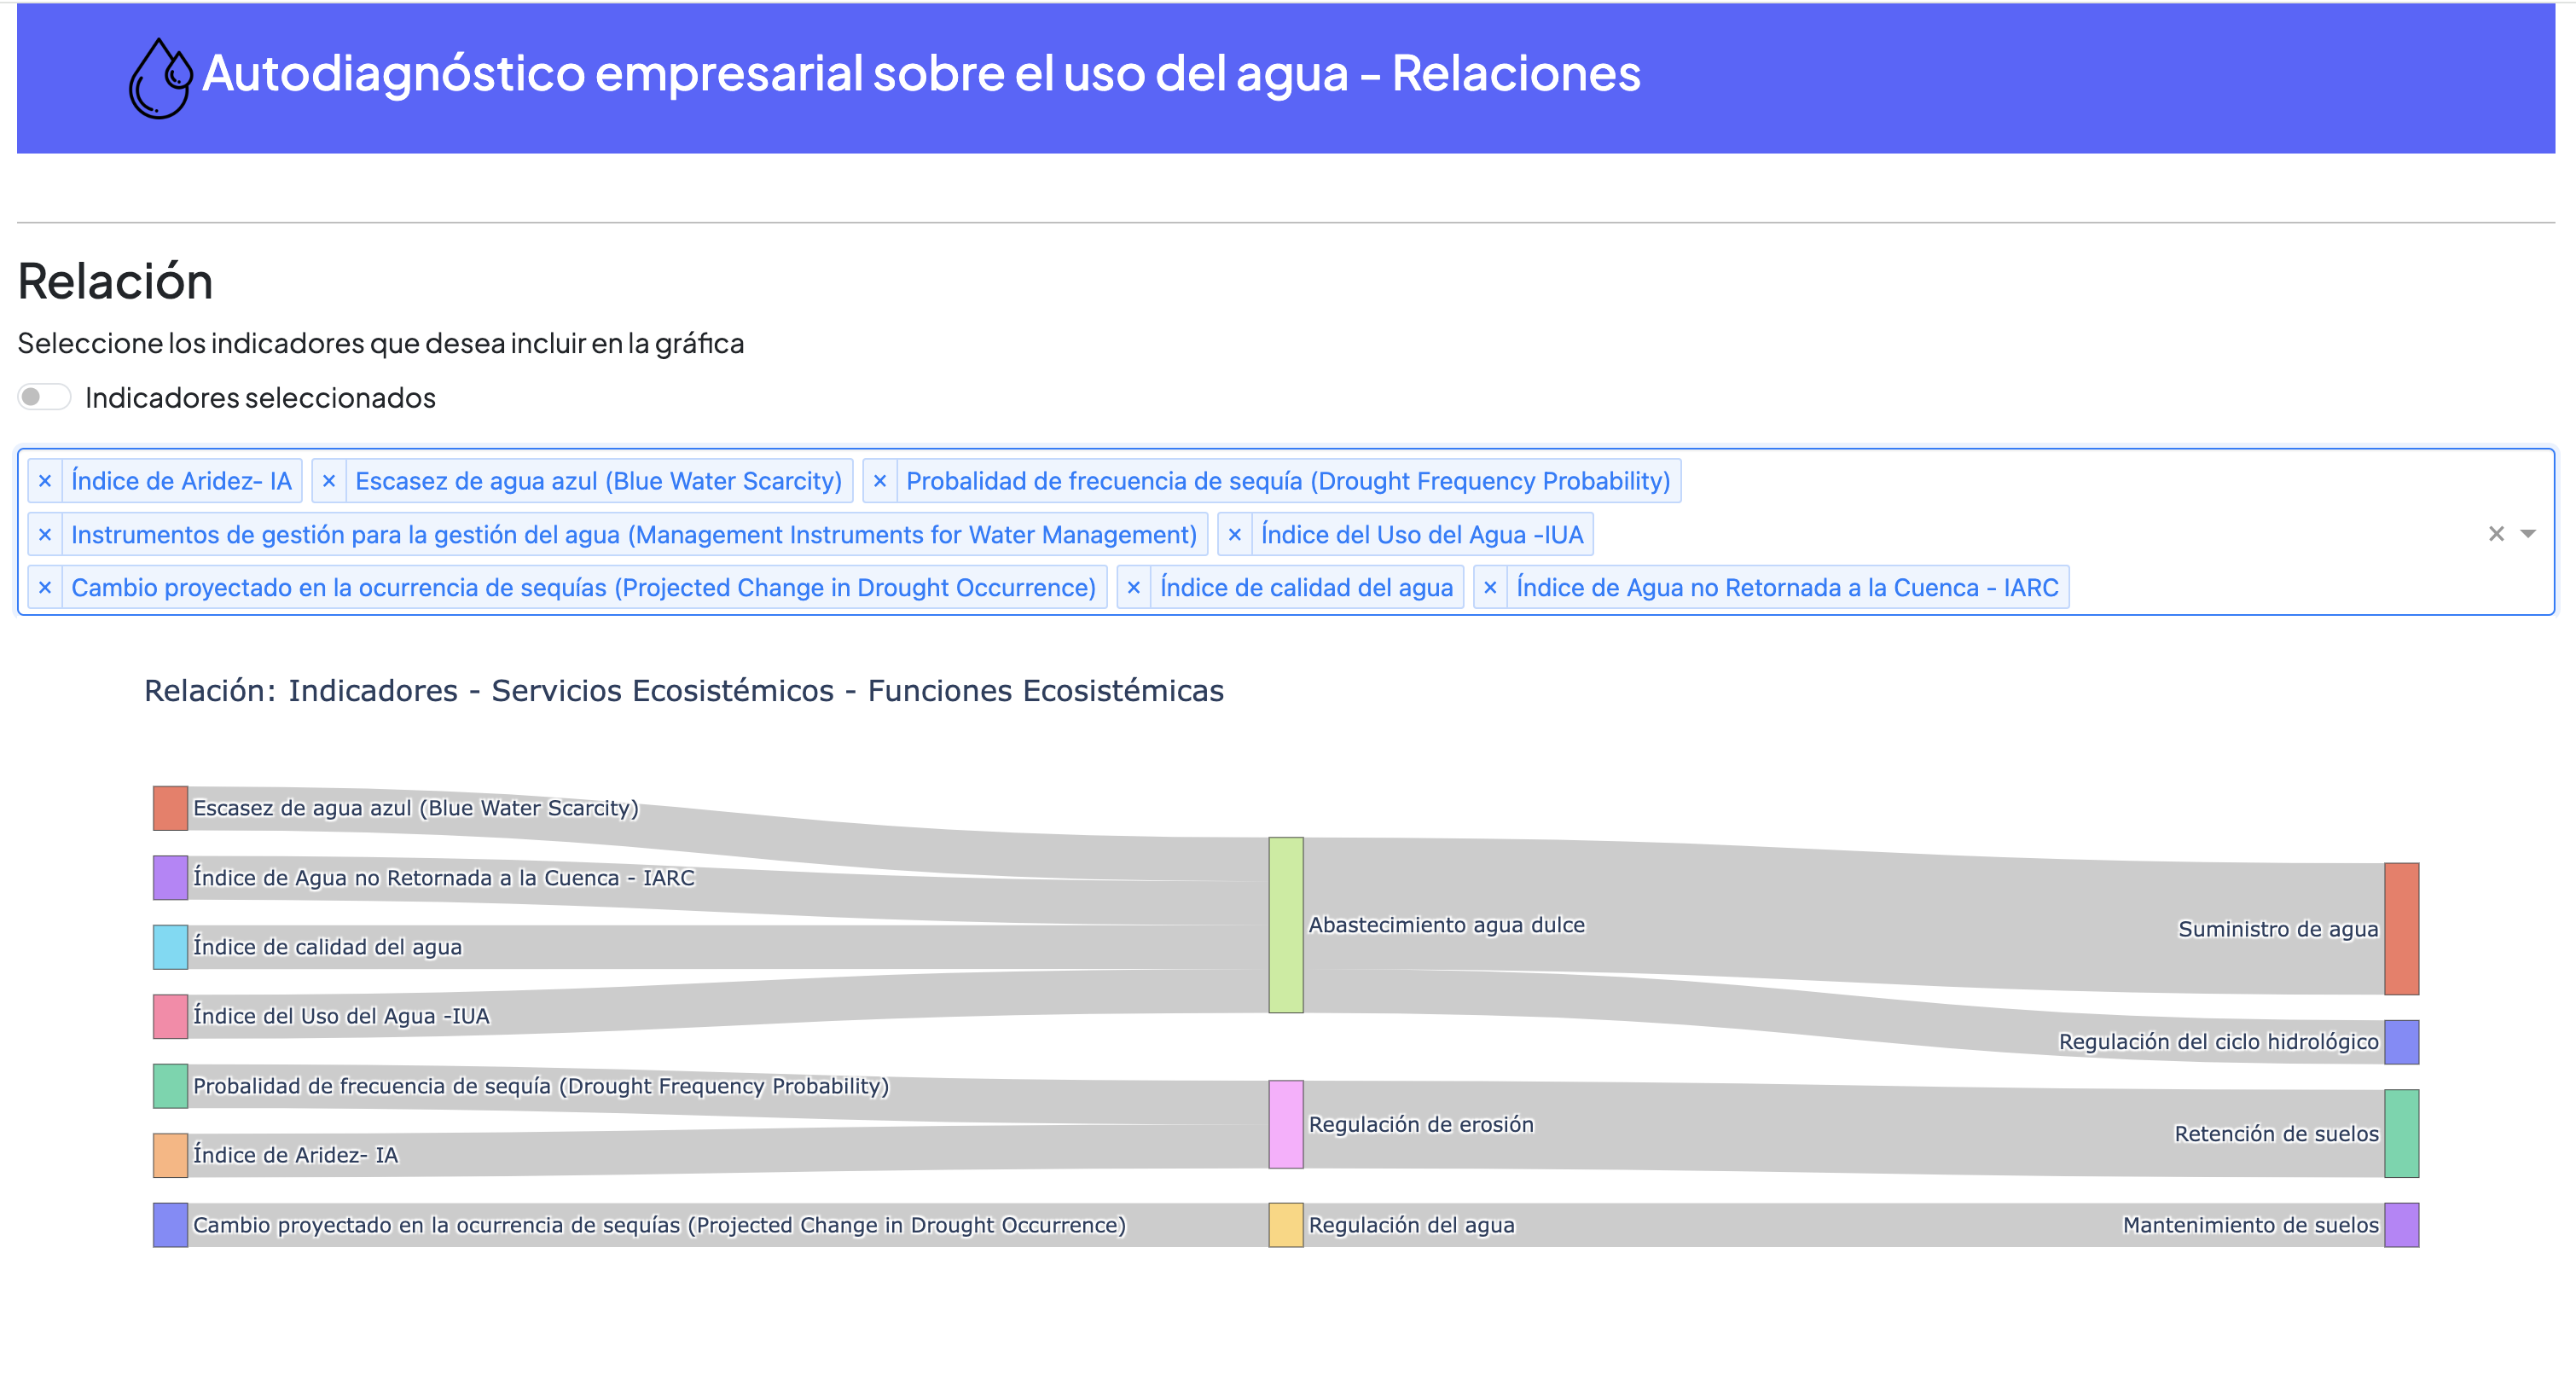
\includegraphics[scale=0.25]{images/99-aplicacion-web/7-relaciones.png}
        \caption{Pantalla donde se muestran las relaciones entre el negocio y los componentes del agua según los indicadores}
\end{figure}

\begin{figure}[H]
        \centering
        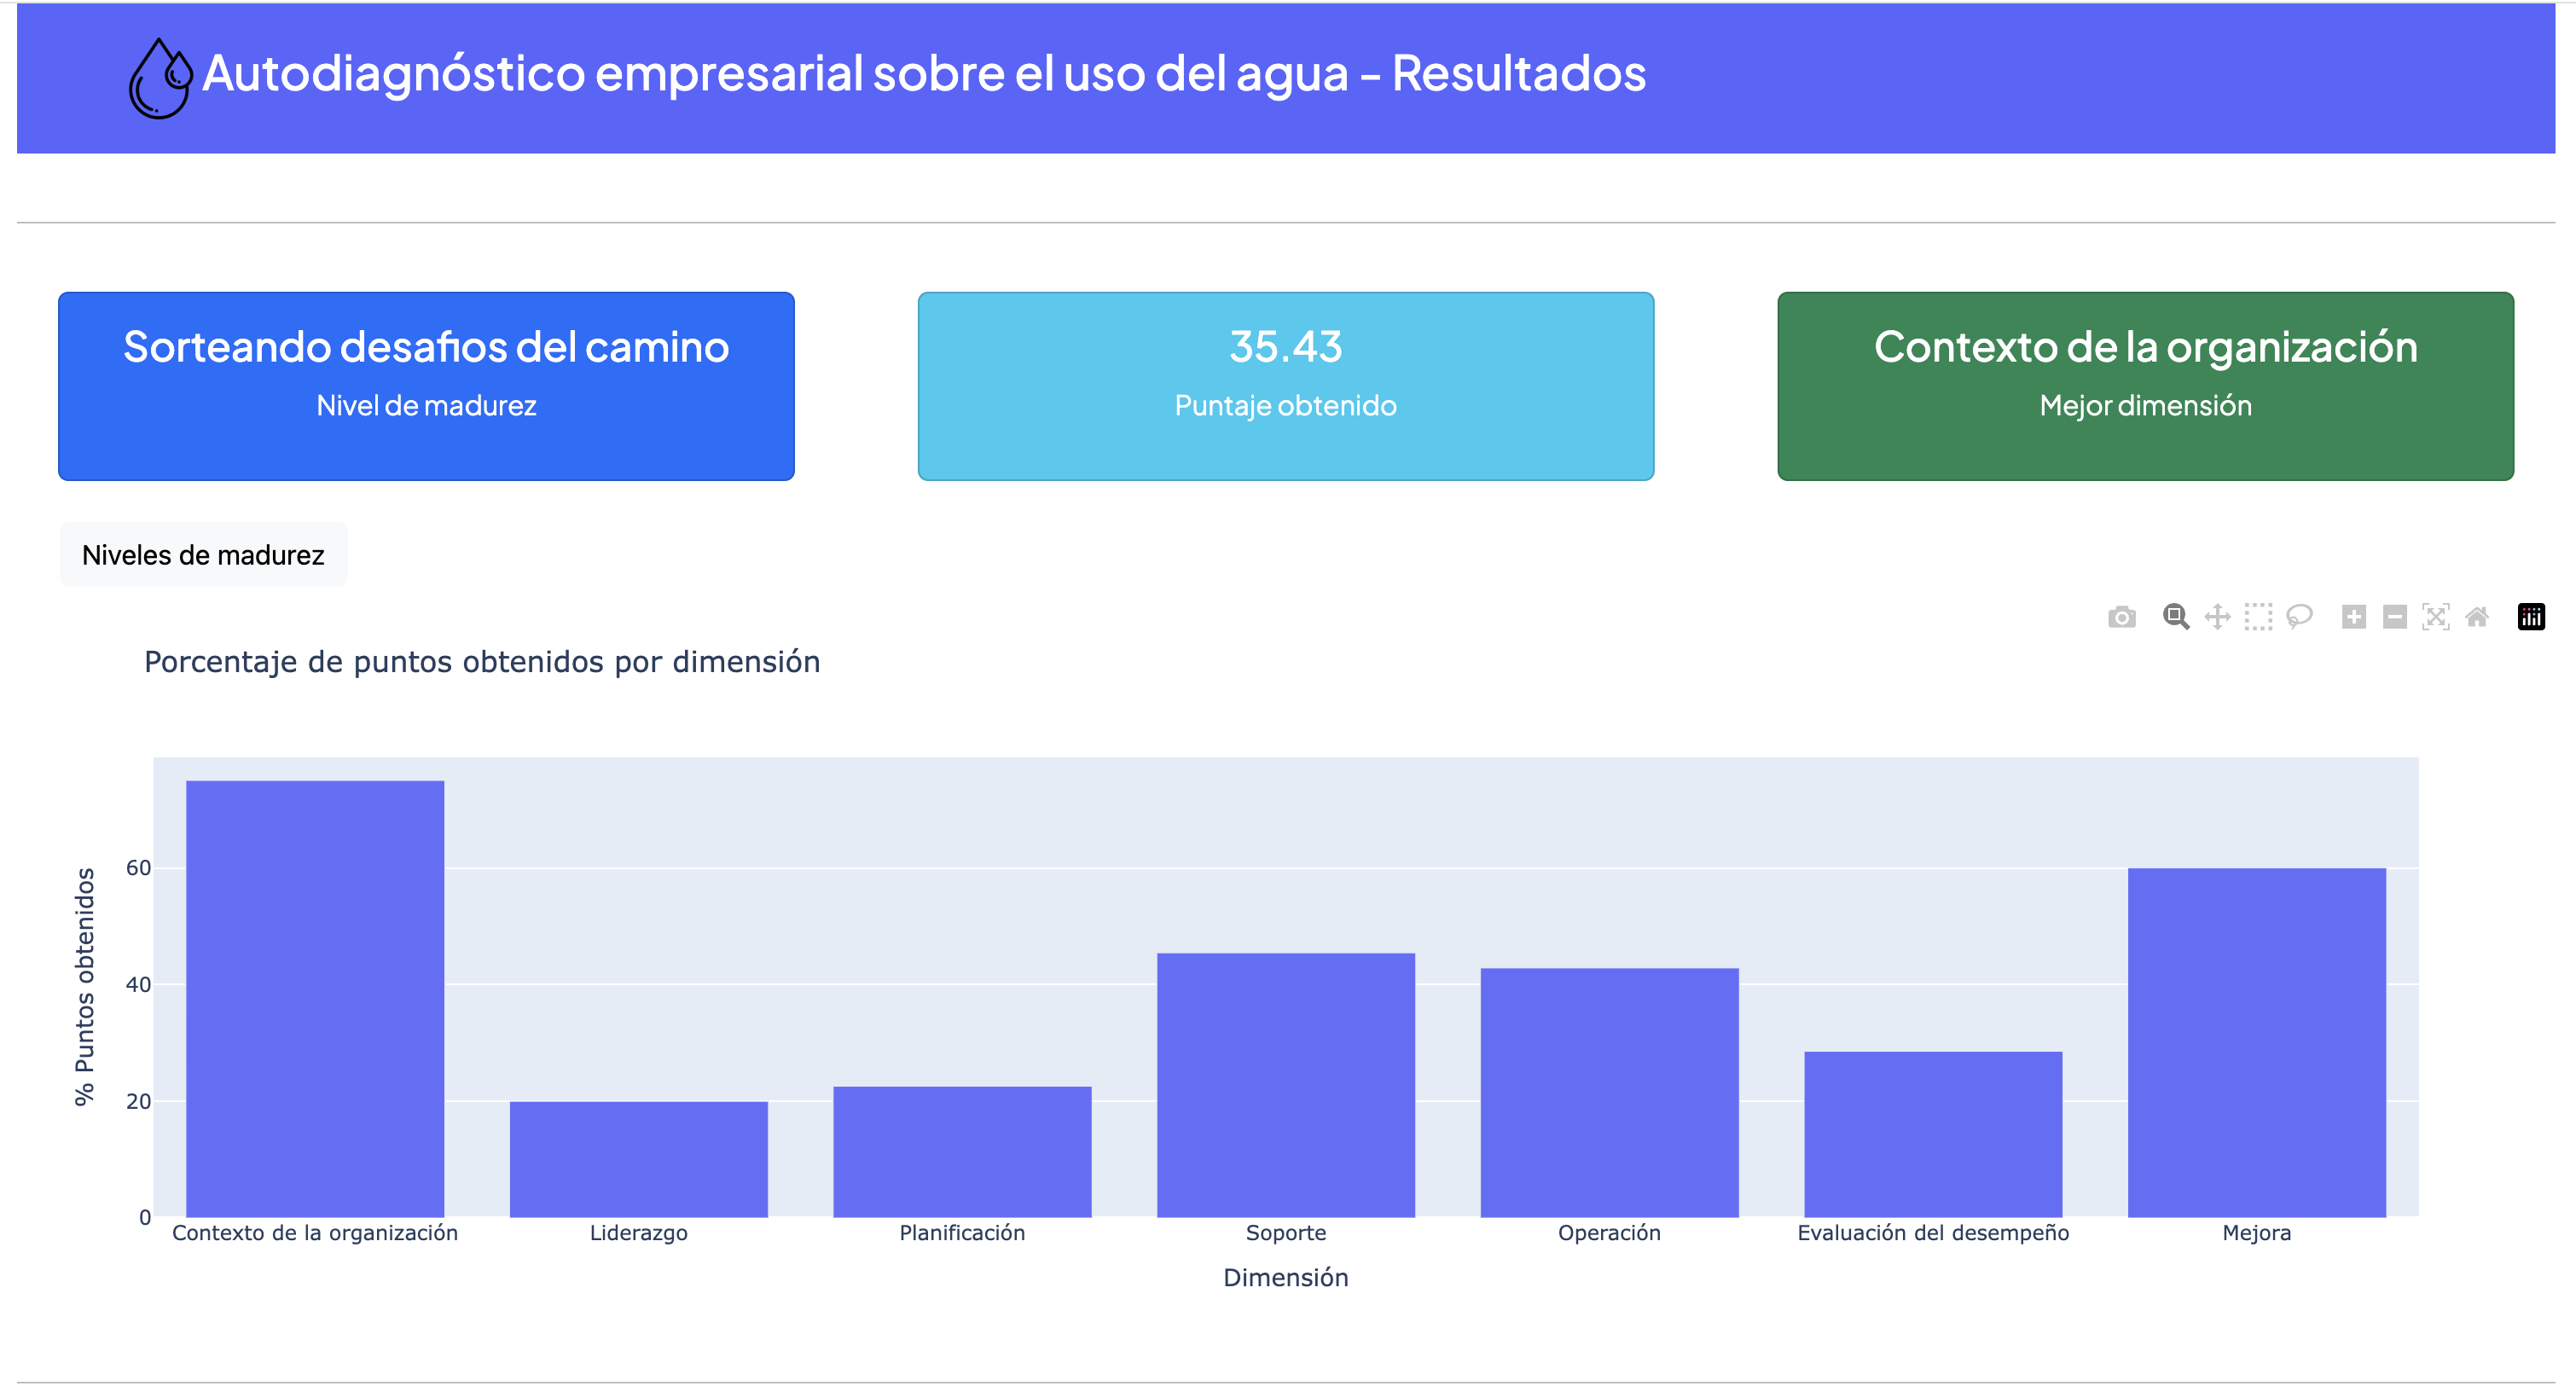
\includegraphics[scale=0.25]{images/99-aplicacion-web/8-mm.png}
        \caption{Resultado: Nivel de madurez de la empresa}
\end{figure}

\begin{figure}[H]
        \centering
        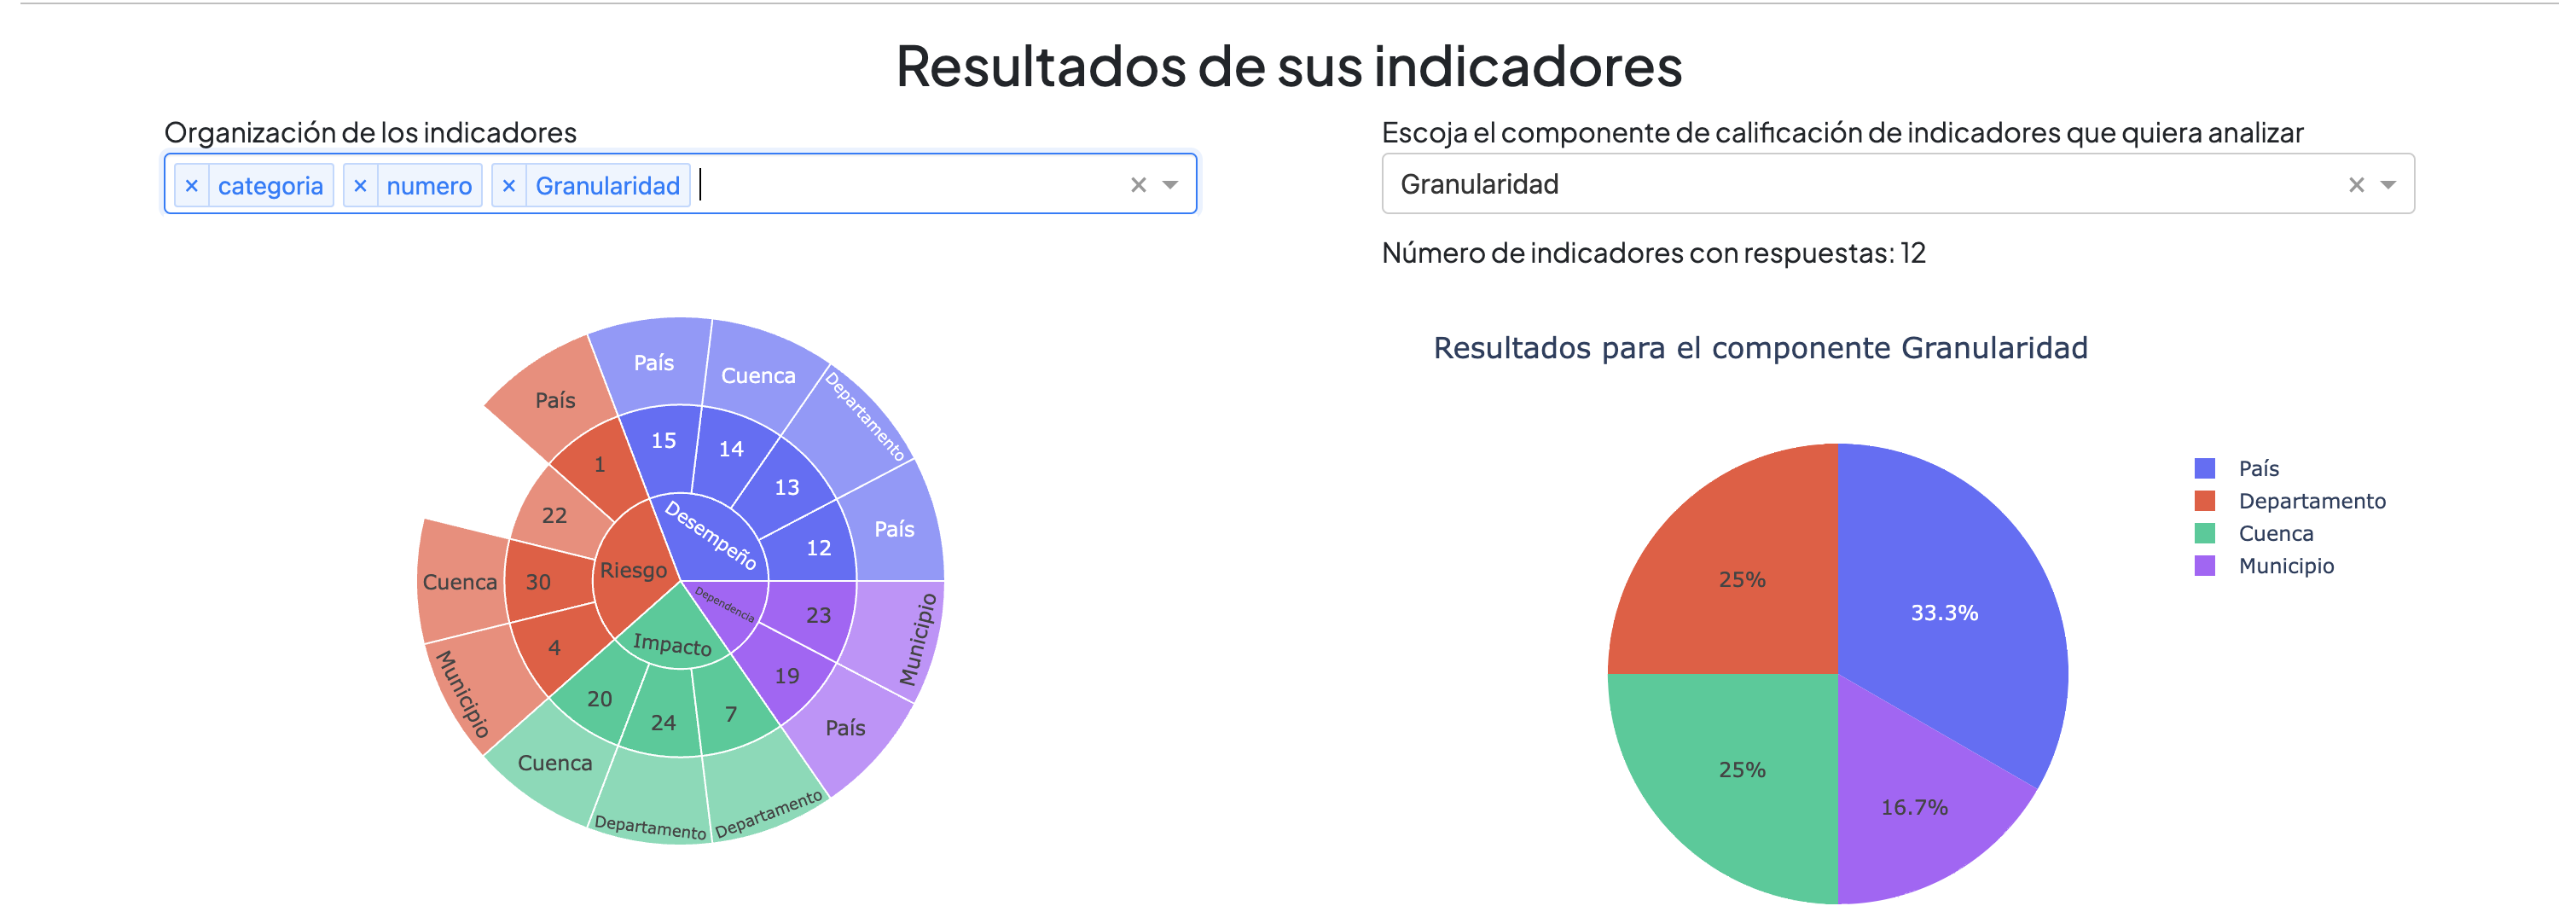
\includegraphics[scale=0.25]{images/99-aplicacion-web/10-respuestas-indicadores.png}
        \caption{Estadísitcas descriptivas de los indicadores seleccionados por la empresa}
\end{figure}